\chapter{Gene Regulatory Networks}
\label{ch_gene_reg_net}


This chapter is based on Ref.\cite{wiki-gene-reg-net}.

Autoregulon networks are
discussed in Chapter \ref{ch-autoregulons}.
Henceforth, we
 will
assume that 
the reader is acquainted
with that chapter.
In particular Section \ref{sec-bio-basis-ar}
of that chapter
explains the biological
underpinnings of 
autoregulon net math.

\begin{figure}[h!]
\centering
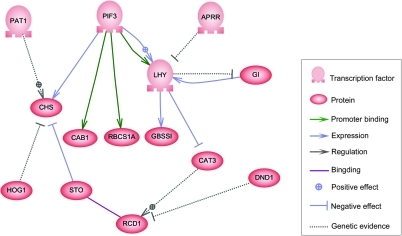
\includegraphics[width=3.5in]
{gene-reg-net/DG_Network_in_Hybrid_Rice.png}
\xymatrix@C=1.3pc{
*+[F*:yellow]{\underline{PAT1}}\ar[dr]|\redoplus
&&*+[F*:yellow]{\underline{P1F3}}\ar[d]
\ar[dl]\ar[drr]|\redoplus\ar[dr]
&&*+[F*:yellow]{\underline{APRR}}\ar[d]|\redominus
&&
\\
&*+[F*:Orchid]{\underline{CHS}}
&*+[F*:Orchid]{\underline{CAB1}}
&*+[F*:Orchid]{\underline{RBCB1A}}
&*+[F*:yellow]{\underline{LHY}}\ar[dr]|\redominus
\ar[d]\ar@/^1pc/[rr]|\redominus
&&*+[F*:Orchid]{\underline{GI}}\ar@/^1pc/[ll]
\\
*+[F*:Orchid]{\underline{HOG1}}\ar[ur]|\redominus
&&*+[F*:Orchid]{\underline{STO}}\ar[ul]|\redominus\ar[dr]
&&*+[F*:Orchid]{\underline{GBSS1}}
&*+[F*:Orchid]{\underline{CAT3}}\ar[dll]|\redoplus
&*+[F*:Orchid]{\underline{DND1}}\ar[dlll]|\redominus
\\
&&&*+[F*:Orchid]{\underline{RCD1}}
&&&
}
\caption{{\bf top:} GRN for hybrid rice, from Ref.\cite{wiki-gene-reg-net}
{\bf bottom:} Same GRN 
as the one on top but in the notation of Chapter \ref{ch-autoregulons}
on Autoregulon Networks.
Yellow boxes are transcription factors (TF). Purple ones are gene expressions.}
\label{fig-rice-gene-reg-net}
\end{figure}





{\bf Gene Regulatory Networks} (GRN) are autoregulon networks 
whose autoregulon nodes are either {\bf gene
expressions} concentrations or {\bf Transcription Factors (TFs)} concentrations.\footnote{This definition of a GRN is my own. 
The conventional definition is
somewhat vague mathematically so 
I changed it to a more mathematically precise and bnet 
friendly one.}




See Fig.\ref{fig-rice-gene-reg-net}
for an example of a GRN.



By a {\bf G2P bnet}\footnote{This is my name for it. I couldn't find a conventional name for it
so I gave it one.}, we will mean a bnet
that maps genotypes (i.e., genes) to phenotypes (i.e., external traits) 

\begin{figure}[h!]
\centering
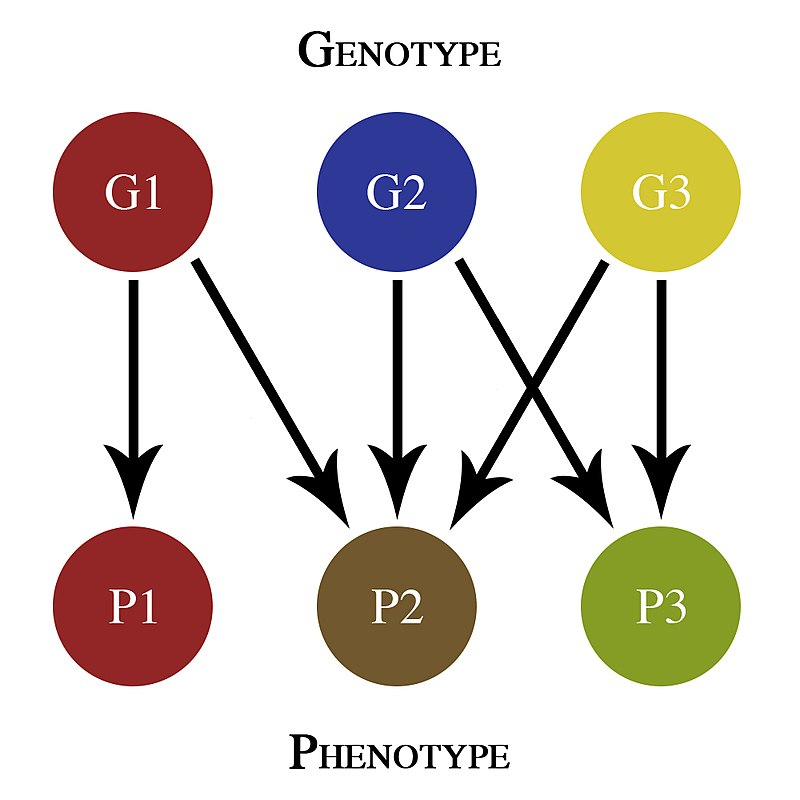
\includegraphics[width=2in]
{gene-reg-net/bnet-more-ways.png}
\caption{G2P bnet. This
one exhibits pleiotropy.}
\label{fig-bnet-more-ways}
\end{figure}

See Fig.\ref{fig-bnet-more-ways} for an example
of a G2P bnet.

When one gene influences more than one external trait, this is called {\bf gene pleiotropy}\footnote{See Wikipedia
article Ref.\cite{wiki-pleiotropy} on pleiotropy.}
(from the Greek words for {\it more-ways}).
Fig.\ref{fig-bnet-more-ways} 
is an example of a G2P bnet that exhibits pleiotropy. 

